%% -*- Lecture -*-

\synctex=1
\documentclass[11pt]{beamer}
\usepackage{microtype}
\usepackage[utf8]{inputenc}
\usepackage[french]{babel}
\uselanguage{French}
\usepackage{minted}

\usepackage{lectureb}
\usetheme{CambridgeUS}

\topic{Processus et Threads}
\author{
  Pablo Oliveira [pablo.oliveira@uvsq.fr]
}



\begin{document}
\maketitle

\begin{slide}{Processus}
\itms{
  \item Un \emph{processus} est une instance en exécution d'un programme
  \item SE modernes sont multi-processus (plusieurs processus en même temps)
  \item Exemples (ces processus peuvent tourner simultanement):
  \ittms{
    \item \texttt{gcc file\_A.c} -- compilateur sur fichier A
    \item \texttt{gcc file\_B.c} -- compilateur sur fichier B
    \item \texttt{vim} -- editeur
    \item \texttt{firefox} -- navigateur
  }
  \item Contre-exemples (implemémentés comme un seul processus):
  \ittms{
    \item Geany: plusieurs tabulations avec des fichiers ouverts
  }
  \item Pourquoi les processus ?
  \ittms{
    \item Isolation
    \item Simples a programmer
    \item Meilleure utilisation CPU et latence
  }
}
\end{slide}

\begin{slide}{Performance}
\itms{
  \item Plusieurs processus améliorent l'utilisation du CPU
  \ittms{
    \item Recouvrement des temps d'attentes et temps de calcul
    \item[] 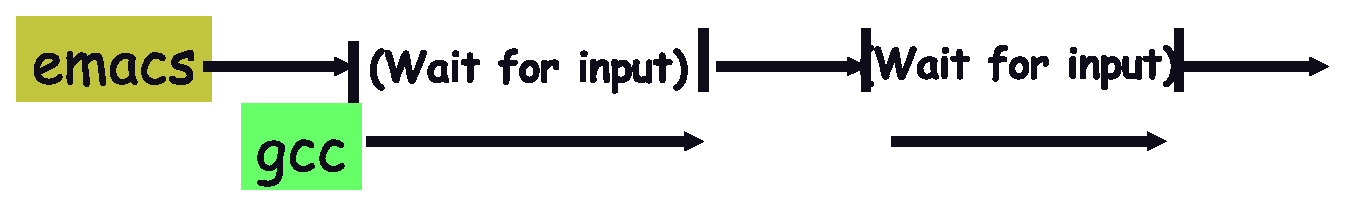
\includegraphics[width=3.5in]{figs/ioparallel}
  }
  \item Plusieurs processus peuvent réduire la latence
  \ittms{
    \item Exécuter $A$ puis $B$ nécessite 100 s pour que $B$ termine \\
     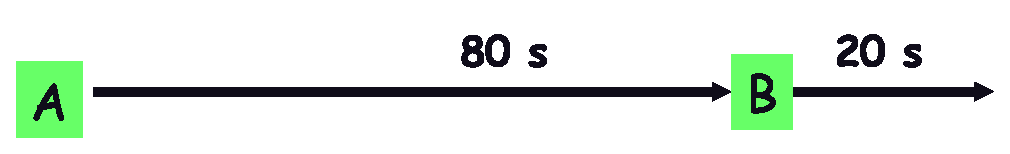
\includegraphics[width=3in]{figs/abseq}
    \item Exécuter $A$ puis $B$ de manière concurrente réduit la latence\\
     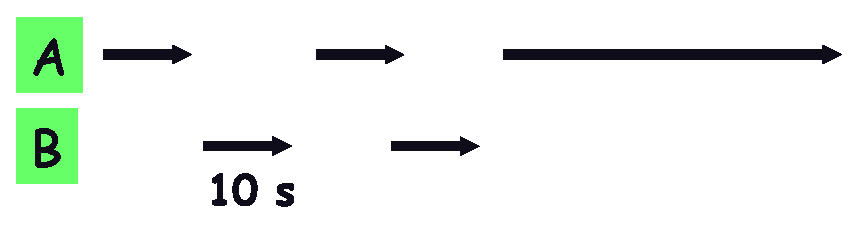
\includegraphics[width=2.5in]{figs/abpar}
   \item $A$ est légèrement plus lent, mais moins que 100 s (excepté si $A$ et
     $B$ utilisent uniquement le CPU).
  }
}
\end{slide}

\begin{slide}{Point de vue du processus}
\hbox{\begin{minipage}{3.1in}
\itms{
  \item Chaque processus a sa propre vue de la machine
  \ittms{
    \item Son propre espace d'adressage
    \item Ses propres fichiers ouverts
    \item Son propre CPU virtuel (par ordonnancement préemptif)
  }
  \item \texttt{*(char *)0xc000} valeur différente entre $P_1$ \& $P_2$
  \item Simplifie énormément la programmation
  \ittms{
    \item \texttt{gcc} n'a pas besoin de se soucier que \texttt{firefox} tourne
  }
}
\end{minipage}
\begin{minipage}{1.2in}
\vspace*{-.3in}
\null
\rightline{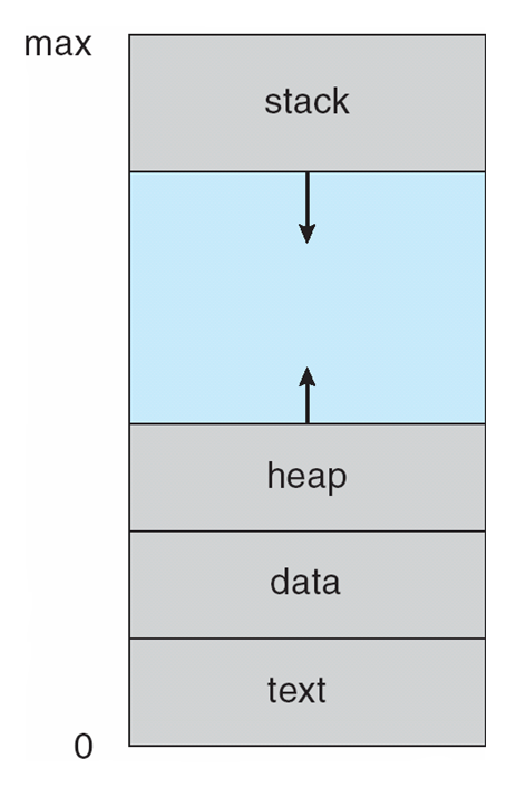
\includegraphics[width=1.3in]{figs/memlayout}}
\end{minipage}}
%\vspace*{-.1in}
\itms{
  \item Parfois l'intéraction entre processus est désirable
  \ittms{
  \item Le plus simple est de communiquer à travers un fichier:  \texttt{vim} édite un fichier,
  \texttt{gcc} le compile
    \item Exemples plus compliqués:  Shell/commande, Gestionnaire de Fenêtres/Application.
  }
}
\end{slide}

\begin{slide}{Communication Inter Processus (IPC)}
\centerline{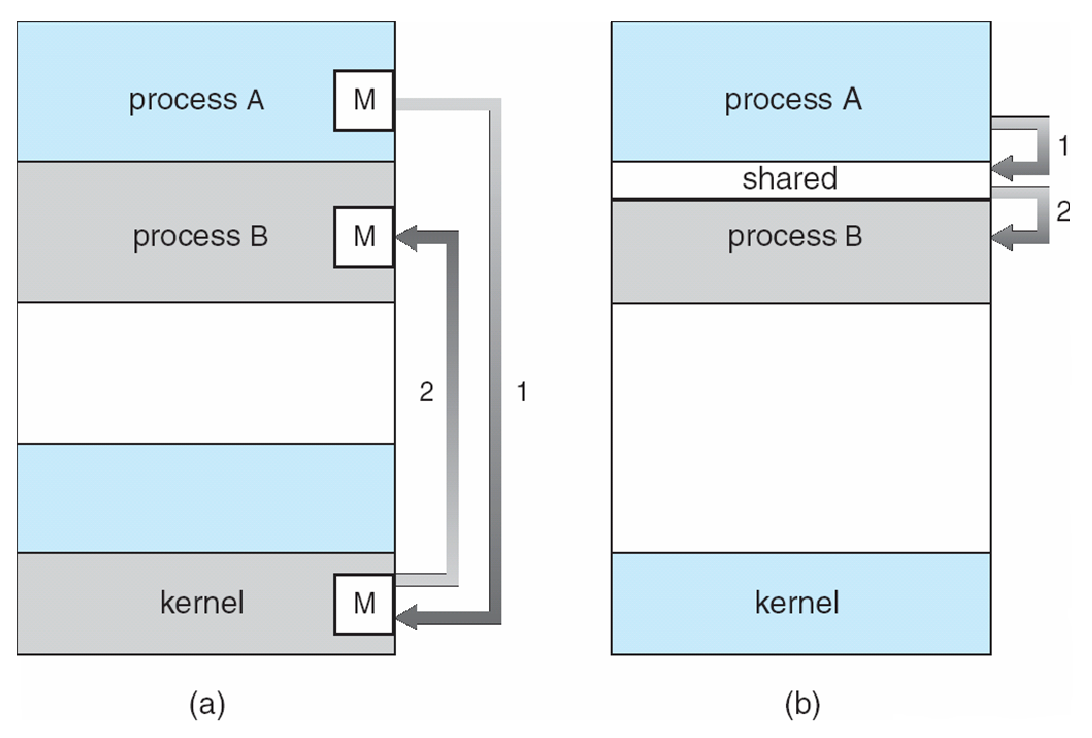
\includegraphics[height=2in]{figs/ipc}}

\small

\itms{
  \item Comment les processus peuvent communiquer en temps réel ?
  \ittms{
    \item[(a)] Par passage de message à travers le noyau
               (eg. signaux asynchrones ou alertes)
    \item[(b)] En partageant une zone commune de la mémoire
  }
}
\end{slide}

\begin{slide}{Plan du cours}
\itms{
  \item Vue utilisateur des processus
  \ittms{
    \item Rappels sur l'interface d'appels systèmes Unix/Linux
    \item Comment créer, tuer et communiquer entre processus
  }
  \item Vue noyau des processus
  \ittms{
    \item Implémentation des processus dans le noyau
  }
  \item Threads
  \item Comment implémenter des threads
}
\end{slide}



\begin{slide}{Créer un processus}
\itms{
  \item \texttt{int fork (void);}
  \ittms{
    \item Crée un processus fils qui est une copie conforme du père
    \item Retourne \textit{l'identifiant (pid)} du fils dans le père
    \item Retourne 0 dans le fils
  }
  \item \texttt{int waitpid (int pid, int *stat, int opt);}
  \ittms{
    \item \texttt{pid} -- processus à attendre, -1 pour n'importe quel processus
    \item \texttt{stat} -- contient la valeur de sortie
    \item \texttt{opt} -- souvent 0 ou \texttt{WNOHANG}
    \item Retourne pid du processus attendu ou -1 en cas d'erreur
  }
  \item \texttt{int wait(int *stat) <=> int waitpid(-1, int *stat, 0);}
}
\end{slide}

\begin{slide}{Terminer un processus}
\itms{
  \item \texttt{void exit (int status);}
  \ittms{
    \item Termine le processus courant
    \item \texttt{status} est retourné dans le \texttt{waitpid} du père
    \item Convention: \texttt{status} est 0 pour une sortie normale
  }
  \item \texttt{int kill (int pid, int sig);}
  \ittms{
    \item Envoie le signal \texttt{sig} au processus \texttt{pid}
    \item \texttt{SIGTERM} tue le processus (le signal peut être intercepté de manière à sortir proprement)
    \item \texttt{SIGKILL} tue le processus (le signal ne peut pas être intercepté)
  }
}
\end{slide}

\begin{slide}{Exécution de programmes}
\vspace*{-.1in}
\itms{
  \item \texttt{int execve (char *prog, char **argv,
	\hbox to0pt{char **envp);\hss}}
  \ittms{
    \item \texttt{prog} -- path du programme à exécuter
    \item \texttt{argv} -- tableau des arguments
    \item \texttt{envp} -- variables d'environnement, e.g.,
	\texttt{PATH}, \texttt{HOME}
  }
  \item Possède plusieurs wrappers plus simples
  \ittms{
  \item \texttt{int execvp (char *prog, char **argv);} \\
    Cherche dans \texttt{PATH} le programme, réutilise l'environnement courant
    \item \texttt{int execlp (char *prog, char *arg, ...);}  \\
    Permet de passer les arguments un par un, doit finir par \texttt{NULL}
  }
  \item Exemple: \texttt{minish.c}
  \ittms{
    \item Boucle qui lit des commandes et les exécute
  }
}
\end{slide}

\begin{slide}{\texttt{minish.c} (simplifié)}
  \small
  \begin{minted}{c}
pid_t pid; char **args;
void doexec () {
  execvp (args[0], args);
  perror (args[0]);
  exit (1);
}
    /* ... main loop: */
    for (;;) {
      parse_next_line_of_input (&args, stdin);
      switch (pid = fork ()) {
      case -1:
        perror ("fork"); break;
      case 0:
        doexec ();
      default:
        waitpid (pid, NULL, 0); break;
      }
    }
  \end{minted}
\end{slide}

\begin{slide}{Manipulation de descripteurs de fichiers}
\itms{
  \item \texttt{int dup2 (int oldfd, int newfd);}
  \ittms{
    \item Ferme \texttt{newfd}, si descripteur valide
    \item Écrase \texttt{newfd} avec une copie conforme de \texttt{oldfd}
    \item Les deux descripteurs partagent l'offset de lecture\\
      (un appel à \texttt{lseek} affecte les deux \texttt{fd})
  }
  \item \texttt{int fcntl (int fd, F\_SETFD, int val)}
  \ittms{
  \item Active (\texttt{val=1}) ou Désactive le mode \textit{close on exec} sur fd.
  \item Le \texttt{fd} ne peut pas être hérité par les programmes lancés avec execv.
  }
  \item Exemple:  \texttt{redirsh.c}
  \ittms{
    \item Loop qui lit une commande et l'éxécute
    \item Reconnaît \texttt{command < input > output 2> errlog}
  }
}
\end{slide}

\begin{slide}{\texttt{redirsh.c}}
  \small
  \begin{minted}{c}
void doexec (void) {
  int fd;
  if (infile) {       /* non vide pour "command < infile" */
    if ((fd = open (infile, O_RDONLY)) < 0) {
      perror (infile);
      exit (1);
    }
    if (fd != 0) {
      dup2 (fd, 0);
      close (fd);
    }
  }

  /* ... pareil pour outfile -> fd 1, errfile -> fd 2 ... */

  execvp (args[0], args);
  perror (args[0]);
  exit (1);
}
\end{minted}
\end{slide}

\begin{slide}{Pipes / Tubes}
\vspace*{-.1in}
\itms{
  \item \texttt{int pipe (int fds[2]);}
  \ittms{
    \item Retourne deux descripteurs dans \texttt{fds[0]} et \texttt{fds[1]}
    \item Une écriture sur \texttt{fds[1]} sera lisible sur \texttt{fds[0]}
    \item Retourne 0 en cas de succès
  }
  \item Opération sur les Tubes
  \ittms{
    \item \texttt{read}/\texttt{write}/\texttt{close} -- comme pour un fichier
    \item Si \texttt{fds[1]} fermé, \texttt{read(fds[0])} retourne 0
    \item Si \texttt{fds[0]} fermé, \texttt{write(fds[1])}:
    \ittms{
      \item Envoie le signal \texttt{SIGPIPE} au processus
      \item Si le signal est ignoré lève la faute EPIPE
    }
  }
  \item Exemple: \texttt{pipesh.c}
  \ittms{
    \item \texttt{command1 | command2 | command3 ...}
  }
}
\end{slide}

\begin{slide}{\texttt{pipesh.c} (simplifié)}
  \small
  \begin{minted}{c}
void doexec (void) {
  while (outcmd) {
    int pipefds[2]; pipe (pipefds);
    switch (fork ()) {
    case -1:
      perror ("fork"); exit (1);
    case 0:
      dup2 (pipefds[1], 1);
      close (pipefds[0]); close (pipefds[1]);
      outcmd = NULL;
      break;
    default:
      dup2 (pipefds[0], 0);
      close (pipefds[0]); close (pipefds[1]);
      parse_command_line (&args, &outcmd);
      break;
    }
  }
\end{minted}
  `$\vdots$'
\end{slide}

\begin{slide}{\hypertarget{wfork}{Pourquoi fork?}}
\itms{
  \item Souvent \texttt{fork} suivi de \texttt{execve}
  \item On pourrait les combiner dans un \emph{spawn} system call
  \item Parfois utile de forker un processus sans \texttt{execve}
  \ittms{
    \item Unix \emph{dump} fait des sauvegardes sur bande
    \item Lorsque la bande est pleine, il faut revenir à un point de sauvegarde
    \item Fork pour revenir à l'état sauvegardé après changement de la bande.
  }
  \item Fork propose une interface très simple
  \ittms{
    \item Plein de choses possibles à faire sur le fils:\\
          manipuler les fd, l'environnement, les limites de ressource, etc.
        \item Pourtant \texttt{fork} ne nécessite aucun argument
  }
}
\end{slide}

\begin{slide}{Lancer des processus sans fork}
\itms{
  \item Sans fork, pléthore d'arguments
  \item Exemple:  Windows
    appel système \href{http://msdn.microsoft.com/en-us/library/ms682425(v=VS.85).aspx}{\texttt{CreateProcess}}

  \ittms{
    \item et
      \href{http://msdn.microsoft.com/en-us/library/ms682429(v=VS.85).aspx}%
           {\texttt{CreateProcessAsUser}},
      \href{http://msdn.microsoft.com/en-us/library/ms682431(v=VS.85).aspx}%
           {\texttt{CreateProcessWithLogonW}},
      \href{http://msdn.microsoft.com/en-us/library/ms682434(v=VS.85).aspx}%
           {\texttt{CreateProcessWithTokenW}},
      \ldots
  }
}

\bigskip

\small
\begin{minted}{c}
BOOL WINAPI CreateProcess(
  _In_opt_       LPCTSTR lpApplicationName,
  _Inout_opt_    LPTSTR lpCommandLine,
  _In_opt_       LPSECURITY_ATTRIBUTES lpProcessAttributes,
  _In_opt_       LPSECURITY_ATTRIBUTES lpThreadAttributes,
  _In_           BOOL bInheritHandles,
  _In_           DWORD dwCreationFlags,
  _In_opt_       LPVOID lpEnvironment,
  _In_opt_       LPCTSTR lpCurrentDirectory,
  _In_           LPSTARTUPINFO lpStartupInfo,
  _Out_          LPPROCESS_INFORMATION lpProcessInformation
);
\end{minted}
\end{slide}


\begin{slide}{Implementation des processus}
\begin{columns}[c]
    \column{.7\textwidth}
\vspace*{-1mm}
  \itms{
  \item Le SE connait la liste des processus
  \ittms{
    \item Process Control Block (PCB)
    \item Appellé \texttt{proc} dans Unix et \texttt{task\_struct} dans
      Linux.
  }
  \item Suit \emph{l'état} du processus
  \ittms{
    \item En Exécution, Prêt, Bloqué, etc.
  }
  \item Inclus l'information sur le contexte du processus
    \ittms{
    \item Banc de registres, traductions d'adresses virtuelles, etc.
    \item Fichier ouverts
  }
  \item D'autres informations sur le processus
  \ittms{
    \item Capabilités (user/group ID), masque de signal, terminal,
    priorité, \ldots
  }
  }
    \column{.33\textwidth}
    \centerline{\input{pcb}}
    \centerline{PCB}
\end{columns}
\end{slide}

\begin{slide}{État d'un processus}
\centerline{\includegraphics[width=3.7in]{procstate}}

\itms{
  \item Les processus sont dans un des états suivants
  \ittms{
    \item \emph{nouveau} \& \emph{terminé} -- en début et en fin de vie
  \item \emph{en exécution} -- en cours d'exécution
  \item \emph{prêt} -- en attente d'être exécuté
  \item \emph{en attente} -- bloqué en attente d'un évenemment (e.g., lecture disque)  }
  \item Quel processus le SE doit-il choisir ?
    \ittms{
    \item Si 0 processus prêt, tourne à vide ou éteint le processeur.
    \item Si $>$1 processus prêts, décision d'ordonnancement
  }
}
\end{slide}

\begin{slide}{Ordonnancement}
\itms{
\item Quel processus exécuter ?
\item Choisir le premier prêt dans la table des processus ?
\ittms{
  \item Coûteux.  Biais de priorité (petits pids)
  \item Deux tables séparées: prêts / en attente
  }
\item FIFO?
\ittms{
  \item File d'attente\\
  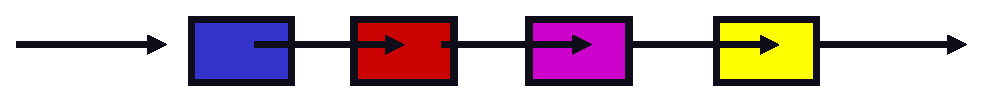
\includegraphics[width=2.5in]{figs/proclist}
}
\item Priorité?
\ittms{
  \item Donner la priorité à certains threads
}
}
\end{slide}

\begin{slide}{Buts de l'Ordonnancement}
\itms{
  \item Compromis entre plusieurs objectifs
  \ittms{
    \item \emph{Équité} -- pas de famine
    \item \emph{Priorité} -- certains processus sont plus importants (QOS)
    \item \emph{Échéances} -- important de faire $x$ (eg. audio) avant une date
    \item \emph{Débit} -- bonne capacité de calcul
    \item \emph{Efficience} -- réduire le surcoût de l'ordonnanceur
  }
  \item Pas de martingale
  \ittms{
    \item Multiobjectifs, on ne peut pas satisfaire tous les critères
    \item Objectifs contradictoires (e.g., priorité vs. équité)
  }
  \item Voir cours sur l'ordonnancement
}
\end{slide}

\begin{slide}{Préemption}
\itms{
  \item Le noyau peut préempter lorsqu'il a le contrôle
  \item Le processus en exécution peut être intérrompu
  \ittms{
    \item Appel système, Faute de page, Instruction illégale
    \item Peut bloquer le processus---e.g., lecture sur disque
    \item Peut débloquer des processus---e.g., fork, écriture sur pipe
  }
\item Timer périodique (interruption horloge)
  \ittms{
  \item Interrompre le processus en exécution si \emph{quantum} consommé
  }
  \item  Interruption matérielle
    \ittms{
    \item Requête disque complète, arrivée d'un paquet réseau
    \item Débloque un processus
    \item qui sera schédulé si ça priorité est plus haute que le processus courant
  }
  \item C'est un changement de contexte
}
\end{slide}

\begin{slide}{Changement de contexte}
\centerline{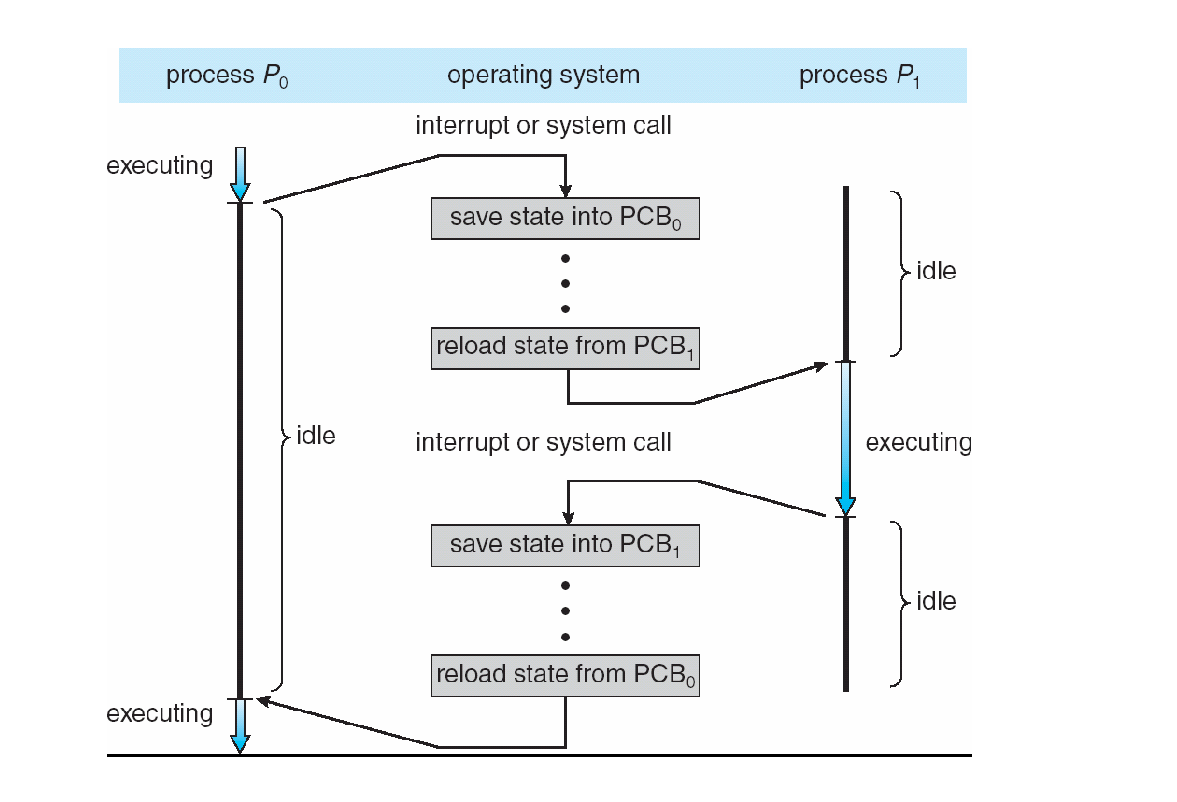
\includegraphics[height=70mm]{figs/switch}}
\end{slide}

\begin{slide}{Détails du changement de contexte}
\itms{
  \item Dépend de l'architecture.  Scénario typique:
    \ittms{
    \item Sauver le compteur ordinal et les registres entiers
    \item Sauver les registres flottants et les registres spéciaux
    \item Sauver les flags conditionnelles
    \item Sauver les traductions d'adresse virtuelles
    }
  \item Coût non négligeable
  \ittms{
    \item Sauver les registres flottants est coûteux\\
    \itttms{
      \item Optimisation: sauvés uniquement si utilisés
    }
  \item Nécessite parfois un flush TLB (cache traduction adresses)\\
    \itttms{
      \item Optimisation: ne pas flusher le TLB avec les traductions du noyau
    }
    \item Cause des miss dans les caches (processus travaillent sur des données différentes)
  }
}
\end{slide}


\begin{slide}{Threads}
\centerline{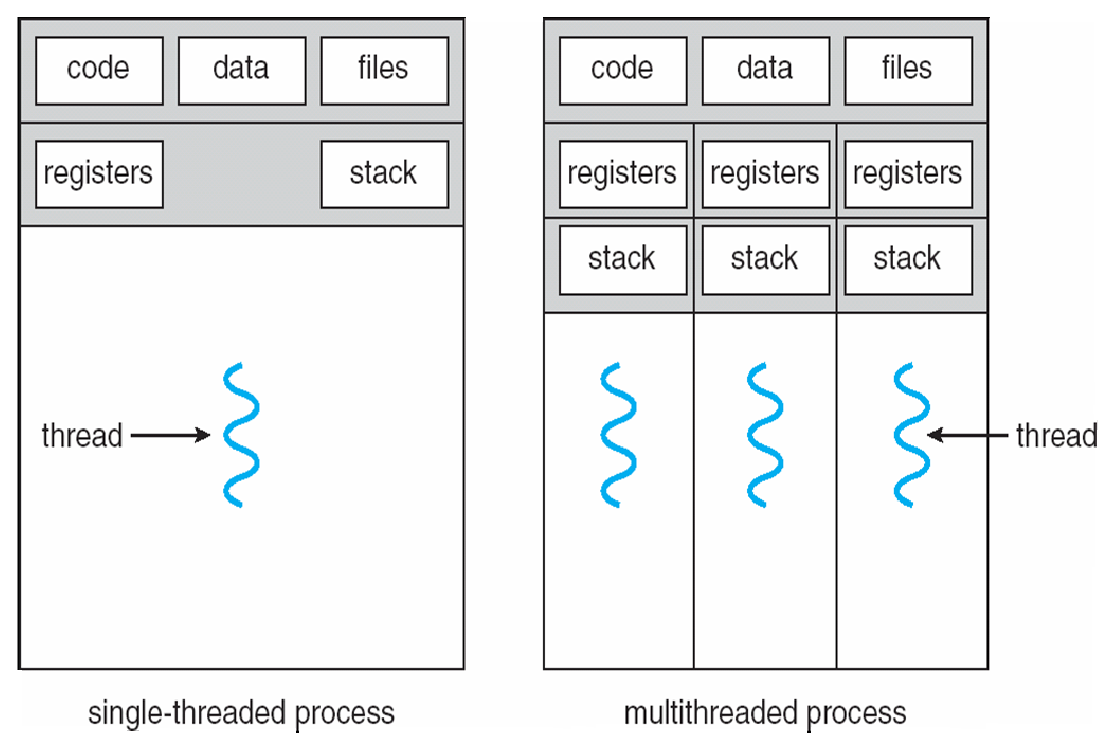
\includegraphics[height=43mm]{figs/thread}}
\itms{
  \item Un thread encapsule un contexte d'execution
  \ittms{
    \item compteur ordinal, pile, registres, \ldots
  }
  \item Programmes simples 1 Thread par Processus
  \item Programmes multi-threads N Threads par Processus
  \ittms{
    \item Les threads se partagent le même espace mémoire
    }
}
\end{slide}

\begin{slide}{Pourquoi les threads ?}
\itms{
  \item Abstraction efficace pour la concurrence
    \ittms{
    \item Plus légers que les processus
    \item Permettent le partage de mémoire (calcul parallèle)
  }
  \item Permettent d'exploiter plusieurs coeurs de calcul
  \item Processus : recouvrement des E/S et du calcul
  \ittms{
    \item Comme pour un SE qui tourne \texttt{emacs} \& \texttt{gcc} simultanement
    \item E.g., un serveur WEB threadé possède un thread par client }
}
\vspace*{-1ex}
\begin{ccode}
        for (;;) {
          fd = accept_client ();
          thread_create (service_client, &fd);
        }
\end{ccode}
\itms{
  \item La plus part des noyaux sont écrits avec des threads
}
\end{slide}


\begin{slide}{Thread POSIX API}
\itms{
  \item \texttt{tid thread\_create (void (*fn) (void *), void *arg);}
  \ittms{
  \item Crée un nouveau thread qui exécute \texttt{fn(arg)}
  }
  \item \texttt{void thread\_exit ();}
  \ittms{
    \item Termine le thread courant
  }
  \item \texttt{void thread\_join (tid thread);}
  \ittms{
    \item Attends la terminaison d'un autre thread
    }
  \item Primitives de synchronization (vues dans le cours 4)
  \item Consulter \cref{sched/readings/birrell.pdf}{[Birell]} pour une bonne introduction
  \item Threads Préemptifs ou Coopératifs
}
\end{slide}


\begin{slide}{Threads Noyau}

\centerline{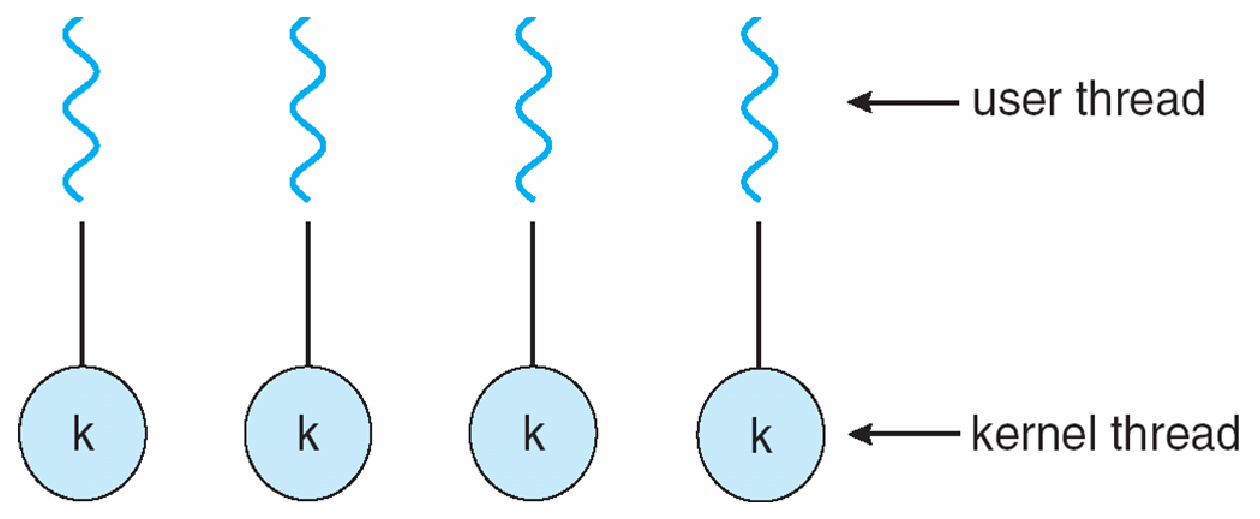
\includegraphics[height=32mm]{figs/kthread}}

\itms{
  \item On pourrait implémenter \texttt{thread\_create} comme un appel système
  \item Pour ajouter \texttt{thread\_create} à un SE où la fonction est absente:
  \ittms{
    \item Prendre pour point de départ un processus Noyau
    \itttms{
      \item Partager le même espace d'adresse, table des fichiers, etc. dans le nouveau processus
    \item Appel système \texttt{clone} sous linux
    }
  }
  \item Plus léger qu'un processus mais assez coûteux tout de même
  }
\end{slide}

\begin{slide}{Limitations des threads noyau}
\itms{
  \item Chaque opération sur le thread passe par le noyau
    \ittms{
    \item creation, sortie, join, synchro, changement de contexte
    \item Sur un laptop: appel système ~ 100 cycles, appel fonction ~ 5 cycles
    \item Conclusion: threads 10x-30x plus lents si implémentés dans le noyau
    }
  \item Hérite des structures de données lourdes des processus
    \ittms{
    \item E.g., taille fixe de pile
  }
}
\end{slide}

\begin{slide}{Threads utilisateurs}
\centerline{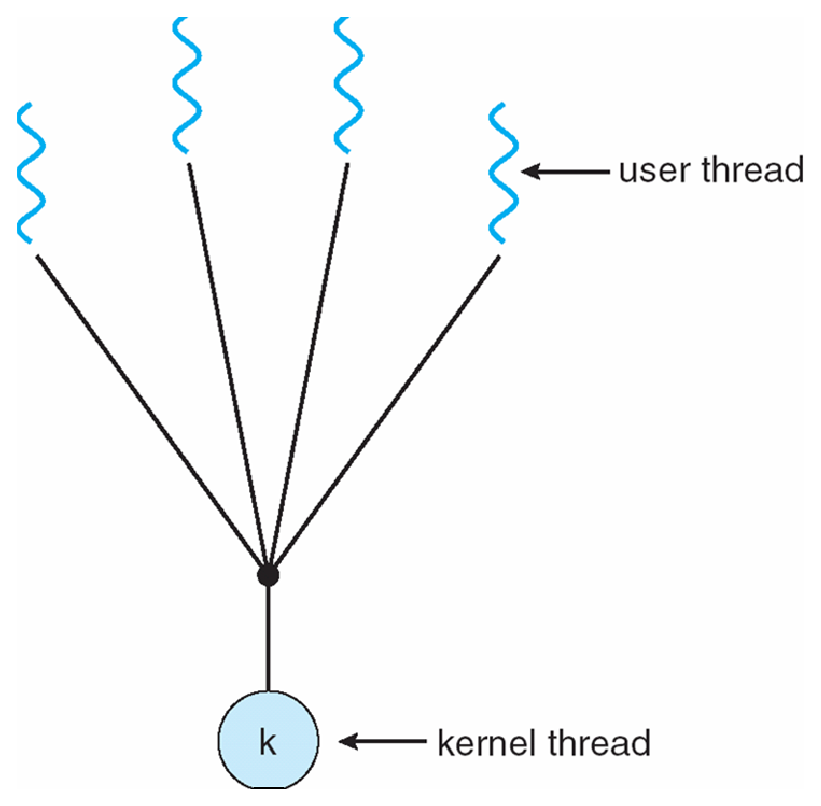
\includegraphics[height=54mm]{figs/uthread}}
\itms{
  \item Les threads peuvent être implémentés en espace utilisateur
    \ittms{
    \item Un seul thread noyau par processus
    \item \texttt{thread\_create}, \texttt{thread\_exit}, etc., simples appels de fonctions
  }
}
\end{slide}

\begin{slide}{Implémentation des threads utilisateur}
\itms{
  \item Allouer une nouvelle pile pour chaque \texttt{thread\_create}
  \item Gérer une pile de threads en attente
  \item Intercepter les appels d'E/S (\texttt{read}/\texttt{write}/etc.)
  \ittms{
    \item Si une opération bloque, changer de thread
    }
  \item Demande un signal d'horloge (\texttt{setitimer})
  \ittms{
    \item Change de thread à chaque réception de signal (preémption)
  }
  \item Example d'un serveur WEB multithréadé  \ittms{
  \item Le thread appelle \texttt{read} pour recevoir une requête
  \item L'appel est intercepté
  \item Si pas de données encore reçues: on passe au thread suivant
  \item À chaque signal d'horloge on vérifie quels threads on reçu des données
  }
  \item Comment changer le contexte de deux threads ?
  }
\end{slide}

\begin{slide}{Présentation des Convention d'appel}
\begin{columns}
\column{.67\textwidth}
\itms{
  \item On sépare les registres en deux groupes
    \ittms{
    \item Les fonctions peuvent écraser les registres \Red{\emph{caller-saved}}\\
      (\texttt{\%eax} [return val], \texttt{\%edx}, \& \texttt{\%ecx})
    \item Mais doivent préserver  les registres \Red{\emph{callee-saved}}
      (\texttt{\%ebx},
      \texttt{\%esi}, \texttt{\%edi}, \texttt{\%ebp} et
      \texttt{\%esp})
  }
  \item \emph{sp} pointe vers le début de la pile
  \item Variables locales dans des registres et sur la pile
  \item Arguments dans des registres caller-saved et sur la pile
    \ittms{
    \item Sur x86, tous les arguments sur la pile
  }
}
\column{.4\textwidth}
\input{stkframe.tex}
\end{columns}
\end{slide}

\begin{slide}{Appels de fonctions}
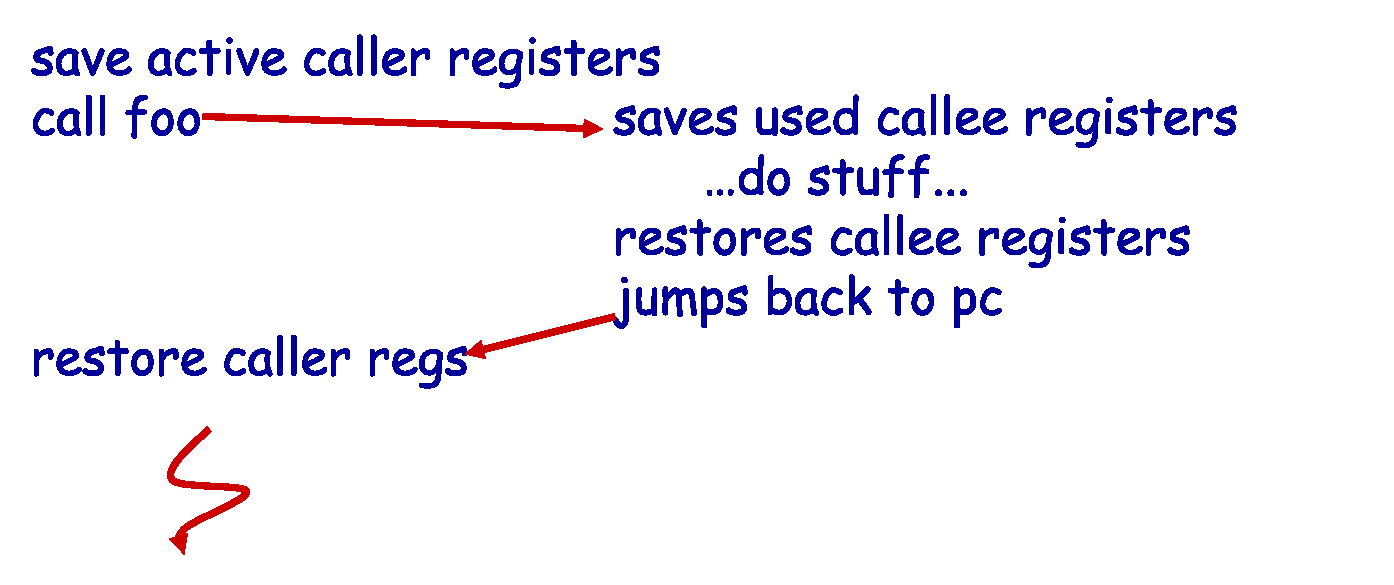
\includegraphics[height=48mm]{figs/proc}
\itms{
  \item État de l'appelant sauvegardé sur la pile
  \ittms{
    \item Adresse de retour, registres caller-saved}
  \item Une partie de l'état est ailleurs
  \ittms{
    \item Registres callee-saved, variables globales, position de la pile}
}
\end{slide}

\begin{slide}{Threads vs.\ fonctions}
\itms{
\item Les threads peuvent être débloqués en un ordre quelconque
  \ittms{
  \item Une pile (LIFO) ne permet donc pas de sauver l'état
  \item Solution générale: une pile par thread
  }
\item Changement de thread moins fréquent que changement de fonction
\ittms{
  \item On ne partitionne pas les registres (Pourquoi ?)
}
\item L'interruption d'une thread peut-être volontaire (\texttt{sleep})
\ittms{
  \item Synchrone: l'appel de fonction sauve une partie de l'état
  \item Asynchrone: le code de changement de contexte sauve tous les registres
}
}
\end{slide}

\begin{slide}{Example d'implémentation de threads utilisateurs}
\itms{
  \item Thread control block (TCB)}
{%
\begin{ccode}
    typedef struct tcb {
      unsigned long md_esp;    /* Pointeur de pile*/
      char *t_stack;           /* Pile */
      /* ... */
    };
\end{ccode}}
\itms{
\item Changement de conxtexte (dépendant de la machine)
    \ittms{
    \item \normalsize\texttt{void thread\_md\_switch (tcb *\Green{current}, tcb
*\Magenta{next});}
  }
\item Initialization d'un thread (dépendant de la machine)
  \ittms{
    \item \normalsize\texttt{void thread\_md\_init (tcb *t,
	void (*fn) (void *),\break\null\qquad void *arg);}
  }
}
\end{slide}

\defverbatim[colored]\threadswitch{\small%
\begin{asm}
pushl %ebp; movl %esp,%ebp             # On sauve epb et esp
pushl %ebx; pushl %esi; pushl %edi     # Sauve callee-saved

movl 8(%ebp),%edx                      # %edx = thread_current
movl 12(%ebp),%eax                     # %eax = thread_next
movl %esp,(%edx)                       # %edx->md_esp = %esp
movl (%eax),%esp                       # %esp = %eax->md_esp

popl %edi; popl %esi; popl %ebx        # Restaure callee-saved
popl %ebp                              # Restaure ebp
ret                                    # continue l'execution
\end{asm}
}

\begin{frame}[fragile]
\frametitle{i386 thread\_md\_switch}
\medskip
\begin{overlayarea}{\textwidth}{56mm}%
\only<1>{\threadswitch}%
\only<2>{\centerline{\input{switch1}}}%
\only<3>{\centerline{\input{switch2}}}%
\only<4>{\centerline{\input{switch3}}}%
\only<5>{\centerline{\input{switch4}}}%
\only<6>{\centerline{\input{switch5}}}%
\end{overlayarea}
\end{frame}

\begin{slide}{Limitations des threads utilisateurs}
\itms{
  \item Ne peuvent pas utiliser plusieurs CPUs
  \item Un appel système bloquant, bloque l'ensemble des threads
    \ittms{
    \item Peut remplacer \texttt{read} pour les connexions reseau
    \item Mais la plus part des SE ne permettent pas l'accès asynchrone au disque
  }
  \item Une faute de page bloque tous les threads
}
\end{slide}

\begin{slide}{Résumé}
\itms{
  \item Threads peuvent être facilement implémentés avec une librairie
    \ittms{
    \item mais les threads noyau ne sont pas forcément la meilleure interface
    }
  \item Les threads sont tout de même très utiles
    \ittms{
      \item Performant pour la plus part des usages
      \item Thread noyaux si l'objectif est d'exploiter la concurrence des E/S
      \item Thread utilisateur pour des application avec beaucoup de
        changements de contexte (e.g,. applications calcul scientifique)
      }
  \item Mais les programmes concurrents sont difficiles à débugger...
}
\end{slide}

\end{document}
